% Section 1: A Classification of Strategic Moves
%-------------------------------------------------------------------------------

\begin{frame}{Unconditional Strategic Moves}
  \textbf{\alert{Commitment}}
  \begin{itemize}
    \item If a player makes an observable and irreversible move to 
    \textbf{limit} their future actions.
    \item ``In the game to follow, I will make a particular move, $X$''
  \end{itemize} 
\end{frame}

% - - - - - - - - - - - - - - - - - - - - - - - - - - - - - - - - - - - - - - - 

\begin{frame}{Unconditional Strategic Moves}
  When does \textbf{\alert{Commitment}} matter?
  \begin{itemize}
    \item When it changes the beliefs of other players
    \item This can rely on the \alert{credibility} of certain commitments.
  \end{itemize} 
\end{frame}

% - - - - - - - - - - - - - - - - - - - - - - - - - - - - - - - - - - - - - - - 

\begin{frame}{Unconditional Strategic Moves}
  \begin{center}
    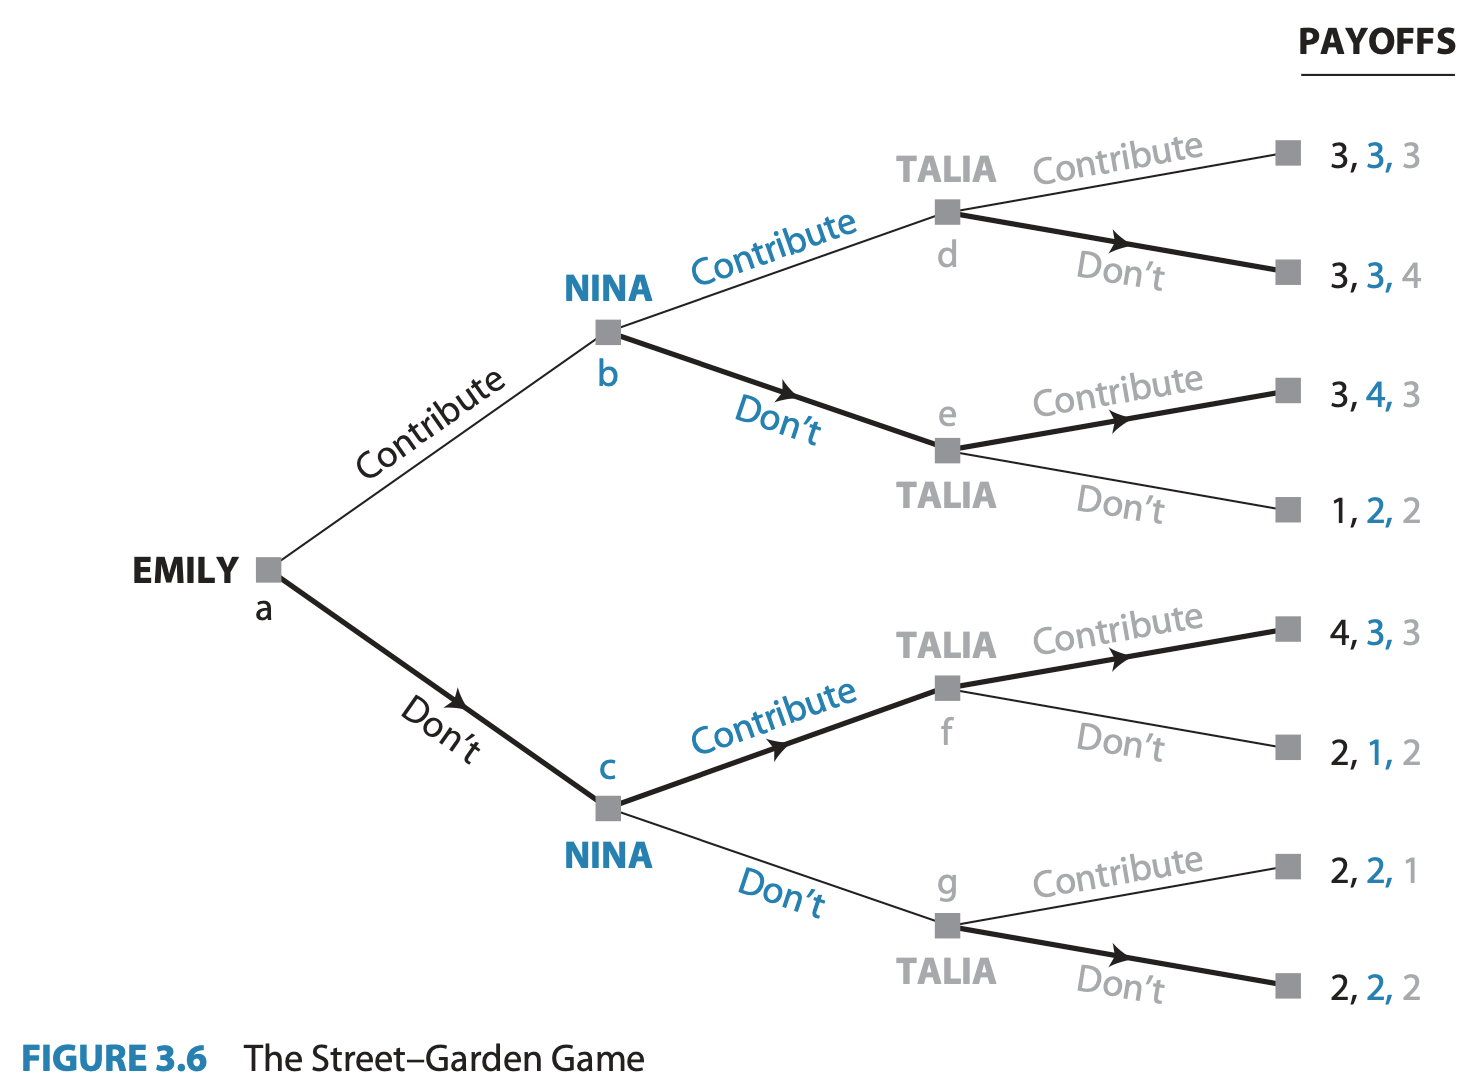
\includegraphics[width=.6\textwidth]{figures/fig3.6.png}
  \end{center}
  Recall that the Street-Garden Game ended with \alert{Emily} \textit{not contributing},
  knowing that both \alert{Nina} and \alert{Talia} \textit{would contribute}.
\end{frame}

% - - - - - - - - - - - - - - - - - - - - - - - - - - - - - - - - - - - - - - - 

\begin{frame}{Unconditional Strategic Moves}
  \begin{center}
    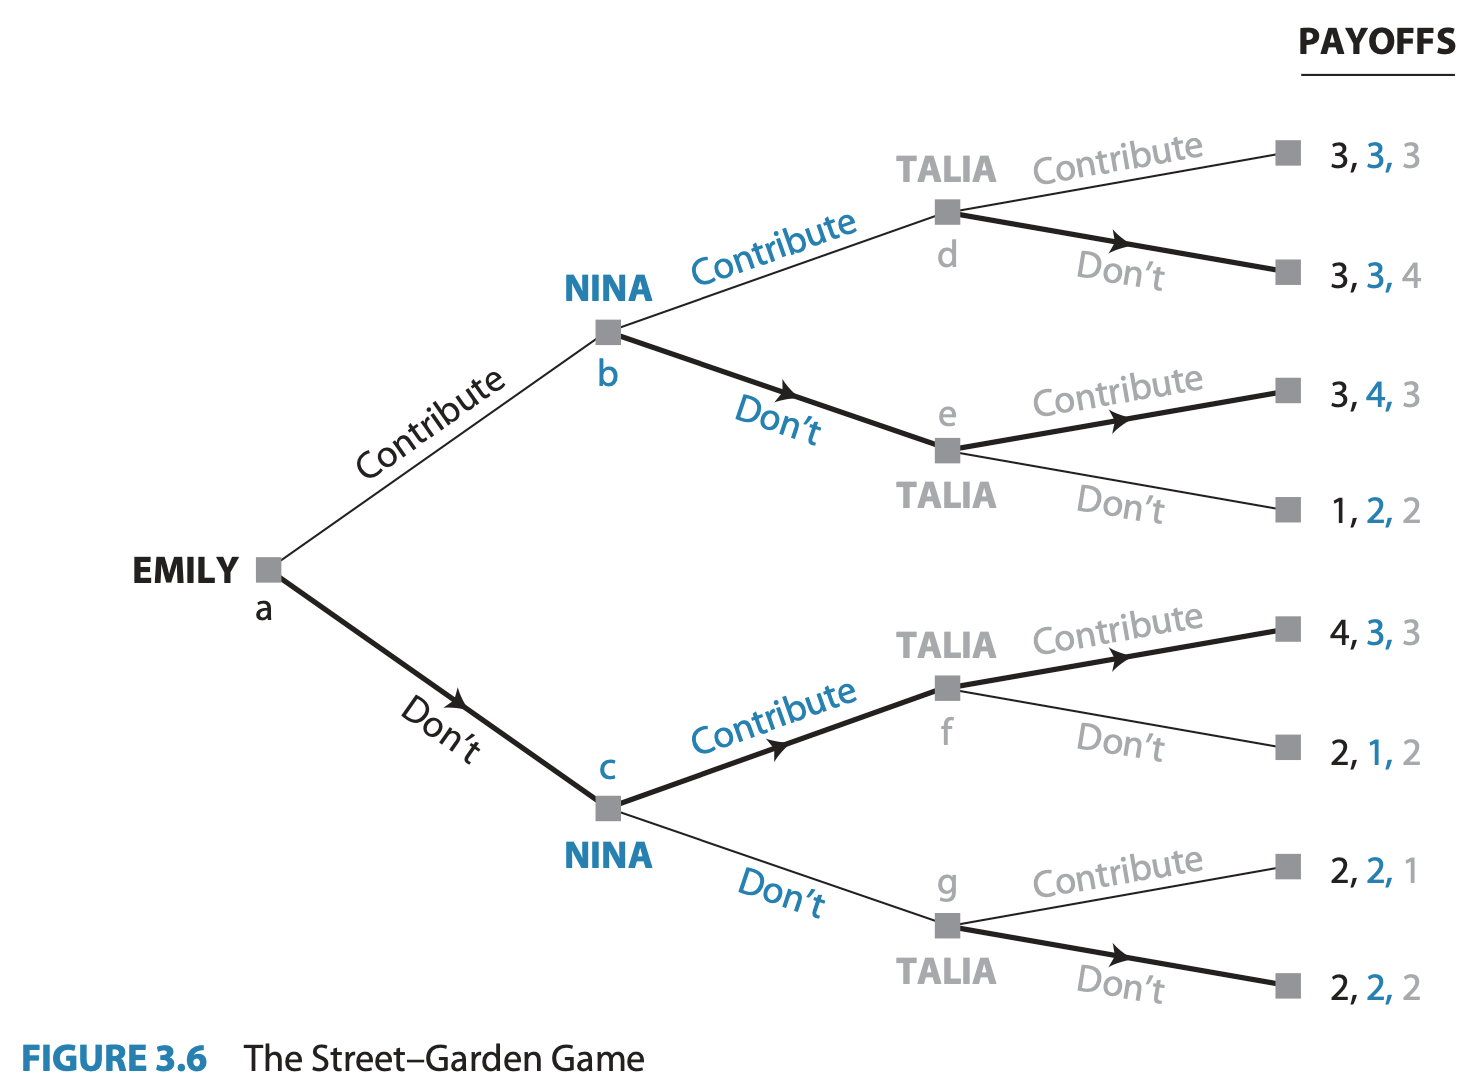
\includegraphics[width=.6\textwidth]{figures/fig3.6.png}
  \end{center}
  But what if either \alert{Nina} or \alert{Talia} can 
  \textbf{commit} to \textit{not contributing}? \\ 
  Maybe \alert{Talia} could let everyone know that she has sunk all of her savings into an expensive home renovation.
\end{frame}

% - - - - - - - - - - - - - - - - - - - - - - - - - - - - - - - - - - - - - - - 

\begin{frame}{Conditional Strategic Moves}
  \textbf{\alert{Response Rules}} 
  \begin{itemize}
    \item If a player makes an observable and irreversible plan that is \textbf{conditional} on another player's actions. 
    \item ``In the game to follow, I will respond to your choices in the following way.
    If you choose $Y_1$, I will do $Z_1$, if you do $Y_2$, I will do $Z_2$, ...''
  \end{itemize}
\end{frame}

% - - - - - - - - - - - - - - - - - - - - - - - - - - - - - - - - - - - - - - - 

\begin{frame}{Conditional Strategic Moves}
  Types of conditional strategic moves
  \begin{itemize}
    \item \alert{Deterrence}: when the first player wants to \textit{stop} another player from making some action
    \item \alert{Compellence}: when the first player wants to \textit{induce} another player to do something 
  \end{itemize}
\end{frame}

% - - - - - - - - - - - - - - - - - - - - - - - - - - - - - - - - - - - - - - - 

\begin{frame}{Conditional Strategic Moves}
  Methods of achieving \textit{deterrence} or \textit{compellence} 
  \begin{itemize}
    \item \alert{Threat}: \\
    ``Unless you do as I want, I will act to make you worse off''
    \item \alert{Promise}: \\
    ``If you do as I want, I will act to make you better off''
  \end{itemize}
\end{frame}

% - - - - - - - - - - - - - - - - - - - - - - - - - - - - - - - - - - - - - - - 

\begin{frame}{Credibility}
  What distinguishes an effective strategic move from \textbf{cheap talk}?
  \begin{itemize}
    \item Any player can promise or threaten anything they like, 
    but whether it works to change other people's behavior depends on its \alert{credibility}
    \item An effective \textit{threat} will be \textbf{costly} to the person doing the threatening.
  \end{itemize}
\end{frame}

% - - - - - - - - - - - - - - - - - - - - - - - - - - - - - - - - - - - - - - - 

\begin{frame}{Split or Steal - Revisited}
  Recall the clip from \href{https://youtu.be/S0qjK3TWZE8}{Golden Balls} we watched with Nick and Ibrahim 
  \begin{itemize}
    \item How would you characterize Nick's strategic move here? 
    \item \alert{Unconditional} or \alert{Conditional}?
    \item \alert{deterrence} or \alert{compellence}?
    \item What parts of Nick's story are \alert{credible}?
  \end{itemize}
\end{frame}
